\documentclass[]{article}
\usepackage{lmodern}
\usepackage{natbib}
\usepackage{float}
\usepackage{amssymb,amsmath}
\usepackage{ifxetex,ifluatex}
\usepackage{fixltx2e} % provides \textsubscript
\ifnum 0\ifxetex 1\fi\ifluatex 1\fi=0 % if pdftex
  \usepackage[T1]{fontenc}
  \usepackage[utf8]{inputenc}
\else % if luatex or xelatex
  \ifxetex
    \usepackage{mathspec}
  \else
    \usepackage{fontspec}
  \fi
  \defaultfontfeatures{Ligatures=TeX,Scale=MatchLowercase}
\fi
% use upquote if available, for straight quotes in verbatim environments
\IfFileExists{upquote.sty}{\usepackage{upquote}}{}
% use microtype if available
\IfFileExists{microtype.sty}{%
\usepackage{microtype}
\UseMicrotypeSet[protrusion]{basicmath} % disable protrusion for tt fonts
}{}
\usepackage[margin=1in]{geometry}
\usepackage{hyperref}
\hypersetup{unicode=true,
            pdftitle={PLSC 508: Replication \& Extension Project},
            pdfauthor={Sam Bestvater},
            pdfborder={0 0 0},
            breaklinks=true}
\urlstyle{same}  % don't use monospace font for urls
\usepackage{graphicx,grffile}
\makeatletter
\def\maxwidth{\ifdim\Gin@nat@width>\linewidth\linewidth\else\Gin@nat@width\fi}
\def\maxheight{\ifdim\Gin@nat@height>\textheight\textheight\else\Gin@nat@height\fi}
\makeatother
% Scale images if necessary, so that they will not overflow the page
% margins by default, and it is still possible to overwrite the defaults
% using explicit options in \includegraphics[width, height, ...]{}
\setkeys{Gin}{width=\maxwidth,height=\maxheight,keepaspectratio}
\IfFileExists{parskip.sty}{%
\usepackage{parskip}
}{% else
\setlength{\parindent}{0pt}
\setlength{\parskip}{6pt plus 2pt minus 1pt}
}
\setlength{\emergencystretch}{3em}  % prevent overfull lines
\providecommand{\tightlist}{%
  \setlength{\itemsep}{0pt}\setlength{\parskip}{0pt}}
\setcounter{secnumdepth}{0}
% Redefines (sub)paragraphs to behave more like sections
\ifx\paragraph\undefined\else
\let\oldparagraph\paragraph
\renewcommand{\paragraph}[1]{\oldparagraph{#1}\mbox{}}
\fi
\ifx\subparagraph\undefined\else
\let\oldsubparagraph\subparagraph
\renewcommand{\subparagraph}[1]{\oldsubparagraph{#1}\mbox{}}
\fi

%%% Use protect on footnotes to avoid problems with footnotes in titles
\let\rmarkdownfootnote\footnote%
\def\footnote{\protect\rmarkdownfootnote}

%%% Change title format to be more compact
\usepackage{titling}

% Create subtitle command for use in maketitle
\newcommand{\subtitle}[1]{
  \posttitle{
    \begin{center}\large#1\end{center}
    }
}

\setlength{\droptitle}{-2em}

  \title{PLSC 508: Replication \& Extension Project}
    \pretitle{\vspace{\droptitle}\centering\huge}
  \posttitle{\par}
    \author{Sam Bestvater}
    \preauthor{\centering\large\emph}
  \postauthor{\par}
      \predate{\centering\large\emph}
  \postdate{\par}
    \date{\today}


\begin{document}
\maketitle

\section{Project Description}

\subsection{Bibliographic reference}

Larson, J.M. and Lewis, J.I., 2017. Ethnic networks. \emph{American Journal of Political Science}, 61(2), pp.350-364.

\textbf{Original Abstract:} Active research on a wide range of political contexts centers on ethnicity's role in collective action. Many theories posit that information flows more easily in ethnically homogeneous areas, facilitating collective action, because social networks among coethnics are denser. Although this characterization is ubiquitous, little empirical work assesses it. Through a novel field experiment in a matched pair of villages in rural Uganda, this article directly examines word-of-mouth information spread and its relationship to ethnic diversity and networks. As expected, information spread more widely in the homogeneous village. However, unexpectedly, the more diverse village's network is significantly denser. Using unusually detailed network data, we offer an explanation for why network density may hamper information dissemination in heterogeneous areas, showing why even slight hesitation to share information with people from other groups can have large aggregate effects.


\subsection{Research extension summary}
\nocite{LarsonLewis_2017}
Larson and Lewis find that the process of information diffusion is more constrained in the ethnically heterogeneous village, despite the fact that it is actually denser than the homogeneous village. In this paper I extend their analysis to explore the specific mechanisms driving this finding. If the social network is characterized by preferential attachment by ethnicity, then we would expect the observed impedance of information diffusion despite the relatively high overall density of the network. In order to test this hypothesis, I fit ERGMs to both networks and compare the tendency toward coethnic preferential attachment.

\subsection{GitHub URL}

\url{https://github.com/bestvater/PLSC508_replication_project}

\newpage

\section{Setup of original study}

Ethnic identity plays an important role in theories of group cohesion and coordination \citep{FearonLaitin_1996}, civil conflict \citep{Varshney_2003}, and electoral patronage/clientelism \citep{Posner_2004}. Common to all these theories is the idea that coethnicity creates informational benefits which facilitate coordination, strengthen ties, and provide access to resources. However, \citet{LarsonLewis_2017} point out that although the coethnic ties are assumed to be stronger than cross-ethnic ties, this assumption has not been systematically studied. Larson and Lewis argue that contrary to \citet{Granovetter_1973}'s classic argument on the ``strength of weak ties," where weak ties are more important for the process of information diffusion due to their ability to bring new information into a cluster, in an ethnically-heterogeneous setting weak cross-ethnic ties are less conducive to information diffusion because even small variations in trust between groups can discourage communication of information, even where cross-ethnic ties exist. Larson and Lewis test this theory using a field experiment conducted on a matched pair of villages in rural Uganda to observe the diffusion of information through word-of-mouth. 

The first village, Abalang, is largely ethnically homogeneous, consisting primarily of members of the Iteso (or Ateso) tribe. The social network of Abalang is depicted in the figure below. This is a directed, unweighted network constructed through the administration of a household census throughout the village.

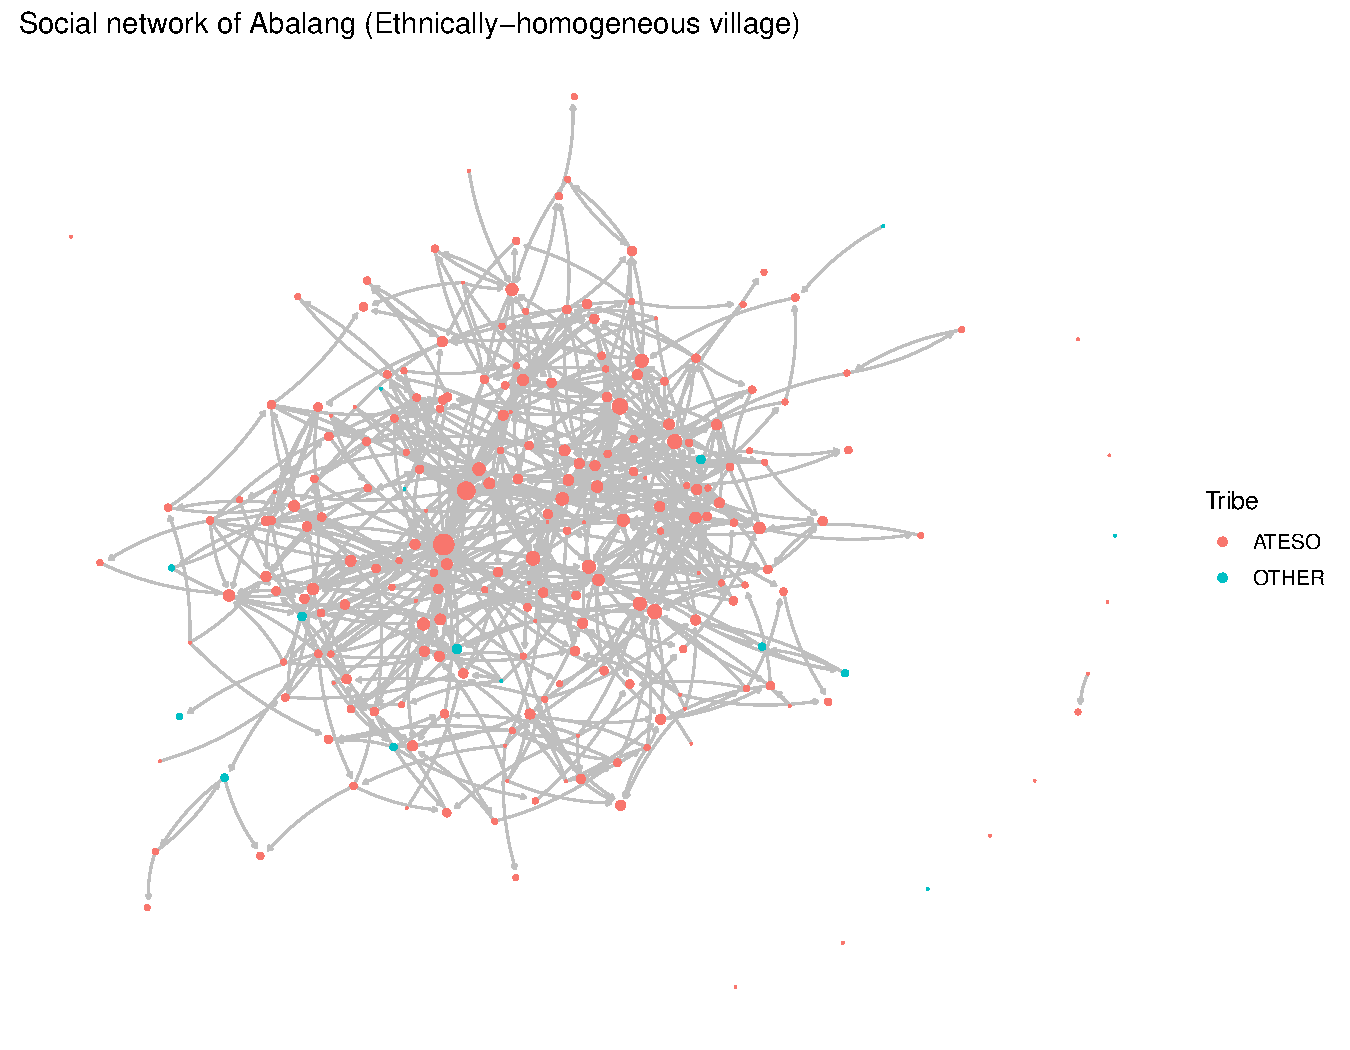
\includegraphics{./figures/abalang_net.pdf}

The second village, Mugana, is comparable to Abalang in most relevant ways. The two villages are only about 2 kilometers apart, are both rural, and are both about the same size (roughly 1,400 residents). Where they differ, however, is in ethnic composition. The Iteso tribe is still the largest group in Mugana, but roughly a third of the village belongs to the Kumam tribe. The social network for Mugana is shown in the figure below:

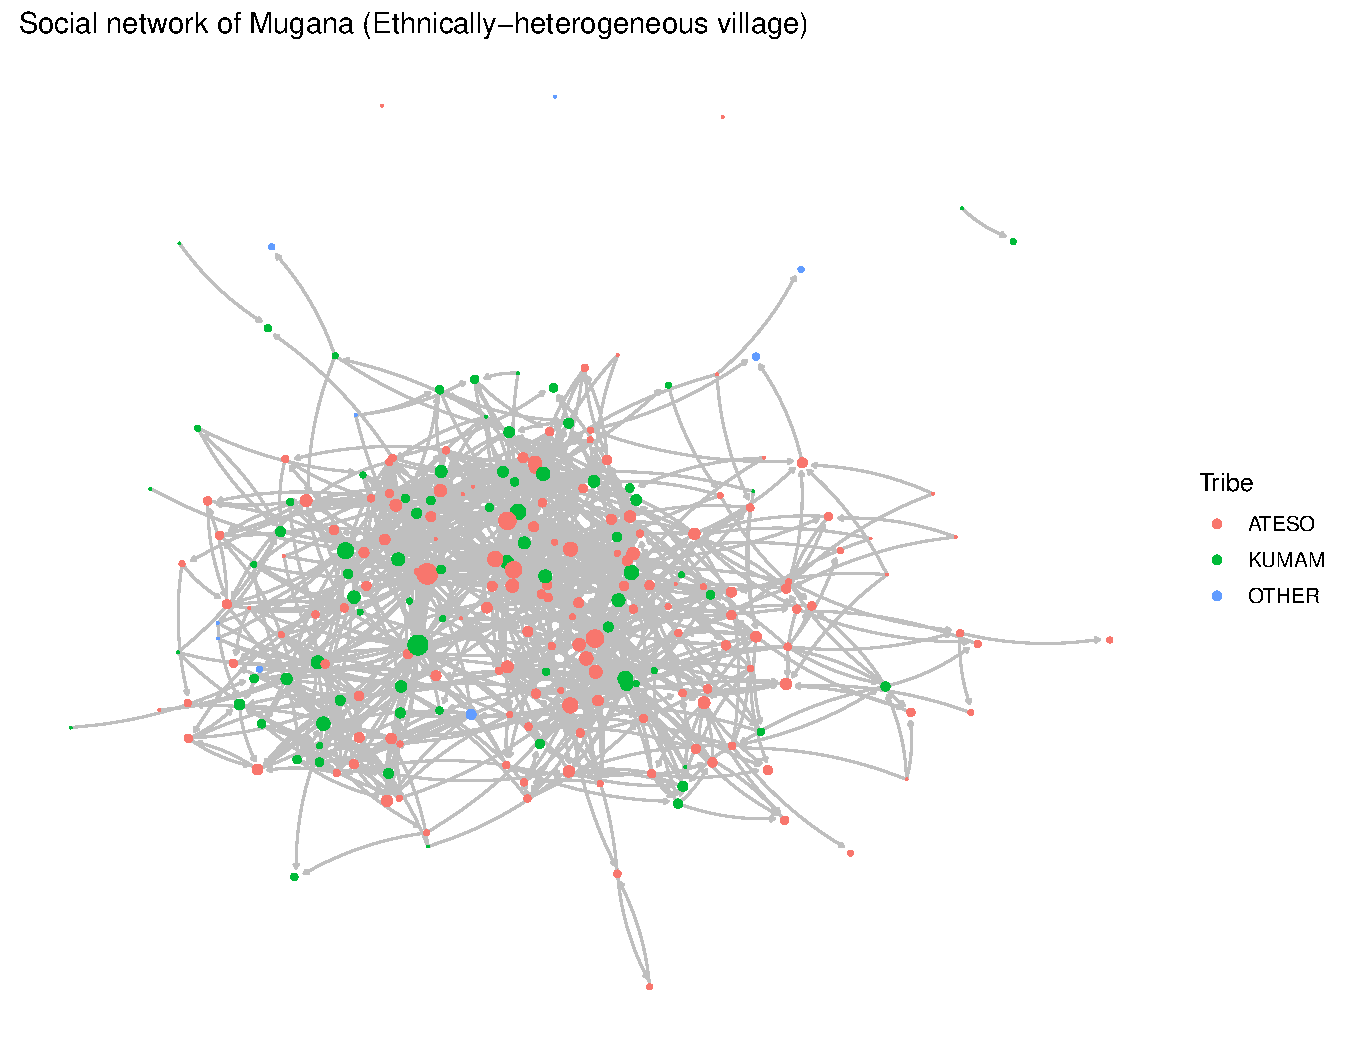
\includegraphics{./figures/mugana_net.pdf}

Notably, when the Mugana network is visualized using the Fruchterman-Reingold force-directed layout algorithm (which tends to capture clustering within networks relatively well) we do not observe much evidence of an obvious ethnic clustering effect within ethnic groups. Some initial descriptive statistics for both networks (as reported in the original paper) appear in Table 1 below:

\begin{table}[H]
\centering
\caption{Network comparisons between Abalang and Mugana}
\begin{tabular}{lll}
\hline
               & \textbf{Abalang} & \textbf{Mugana} \\ \hline
Total Nodes    & 216              & 234             \\
Total Links    & 660              & 965             \\
Reciprocal     & .20              & .21             \\
Average Degree & 6.1              & 8.2             \\
Density        & .014             & .018           \\ \hline 
\end{tabular}
\end{table}

The distribution of ethnic identities in Mugana and Abalang is summarized visually in the figure below.

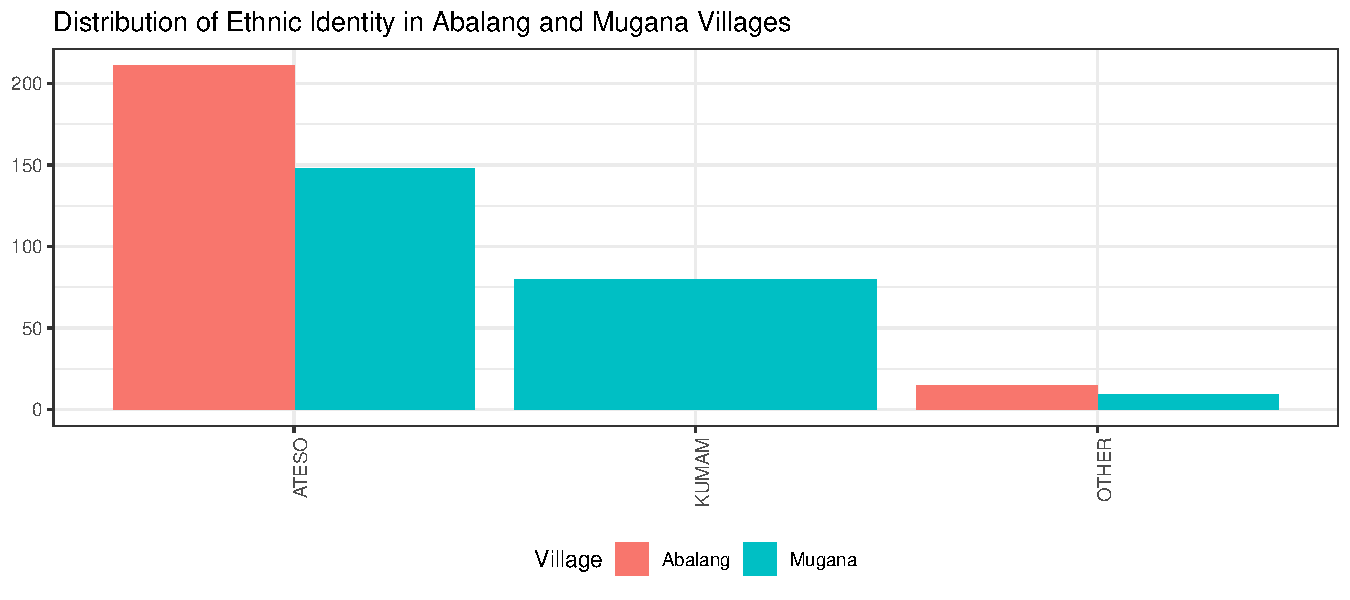
\includegraphics{./figures/ethnicity.pdf}

In order to capture the effect of cross-ethnic weak ties on information diffusion, Larson and Lewis implemented a field experiment in Mugana and Abalang, where households were randomly chosen to receive novel information about an upcoming event of interest from a Ugandan research assistant. Then, when the research team later visited the villages to survey residents and compile the social network data, respondents were asked if they had heard about the event, and if they had attended it. 

\section{Replication of original results}

The fundamental result from Larson and Lewis' field experiment was that in ethnically-homogeneous Abalang, information about the event reached the majority of residents from an initial seed of only 7 households. In ethnically-heterogeneous Mugana, by contrast, the information spread to fewer than 25 other nodes in the network, despite originating from a larger seed of 10 households. These descriptive results are presented in the figures below:

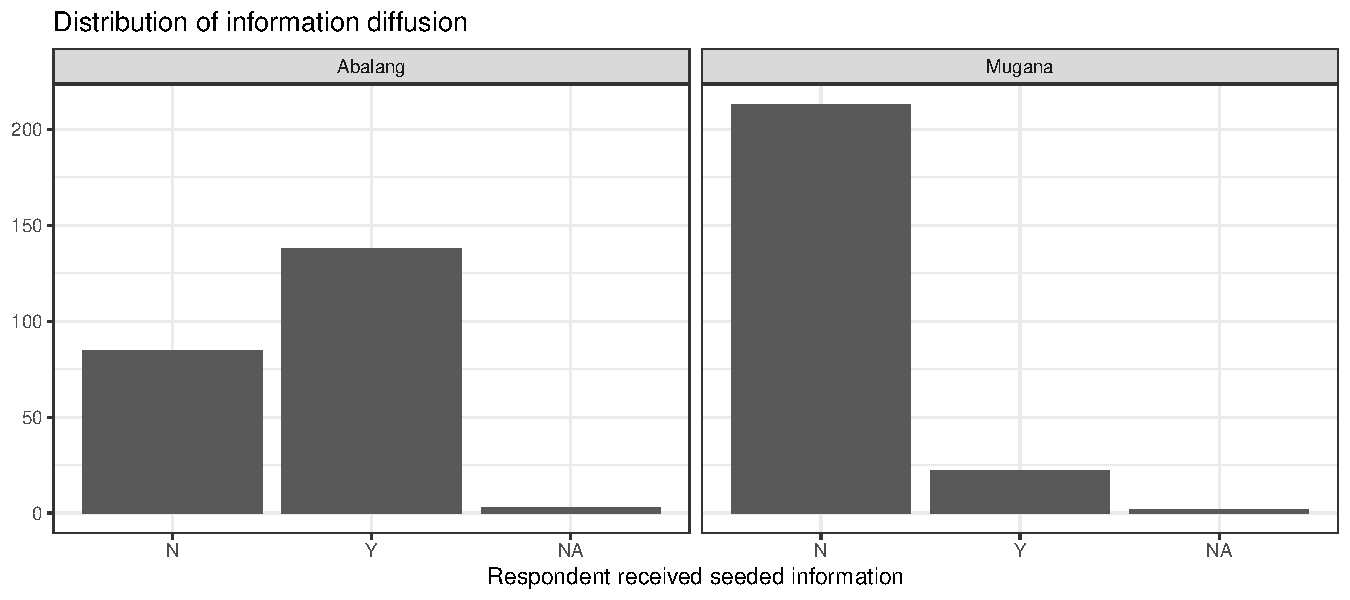
\includegraphics{./figures/info_diffusion.pdf}

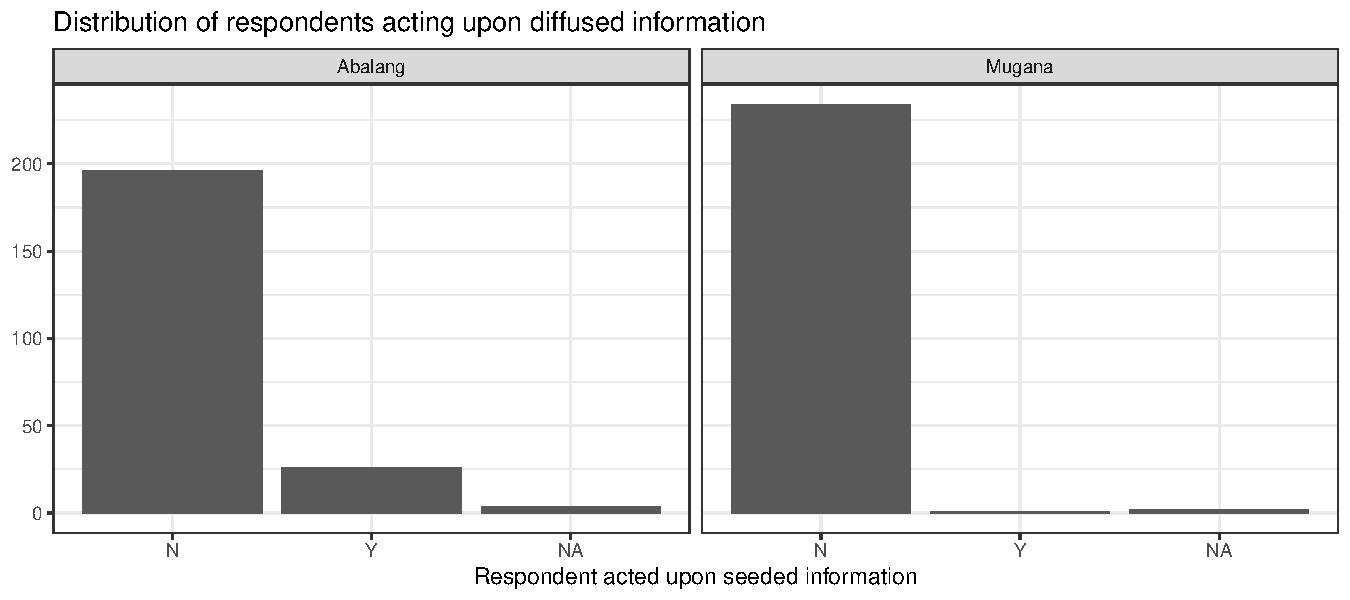
\includegraphics{./figures/info_action.pdf}

Larson and Lewis confirm their belief that information about the event spread primarily through word-of-mouth, quotidian exchanges along the social network through a series of logistic regressions on the Abalang sample which regress whether or not a respondent heard about the event on a number of demographic characteristics and network measures, replicated in Table 2 below. The critical variable here is \textit{PHoodHear} in specifications (3) and (4), which measures the proportion of first-degree neighbors in an individual's social network who also heard about the event. Having a high proportion of neighbors who heard about the event is strongly and significantly predictive of an individual hearing about it themselves.



% Table created by stargazer v.5.2.2 by Marek Hlavac, Harvard University. E-mail: hlavac at fas.harvard.edu
% Date and time: Wed, Apr 29, 2020 - 14:27:36
\begin{table}[H] \centering 
  \caption{Predicting whether respondent heard about the event} 
  \label{} 
\footnotesize 
\begin{tabular}{@{\extracolsep{5pt}}lcccc} 
\\[-1.8ex]\hline 
\hline \\[-1.8ex] 
 & \multicolumn{4}{c}{\textit{Dependent variable:}} \\ 
\cline{2-5} 
\\[-1.8ex] & \multicolumn{4}{c}{Hear} \\ 
\\[-1.8ex] & (1) & (2) & (3) & (4)\\ 
\hline \\[-1.8ex] 
 Gender & 1.044$^{***}$ & 1.175$^{***}$ & 0.900$^{**}$ & 0.995$^{***}$ \\ 
  & (0.350) & (0.363) & (0.364) & (0.375) \\ 
  & & & & \\ 
 Age & 0.001 & 0.003 & 0.004 & 0.004 \\ 
  & (0.010) & (0.010) & (0.011) & (0.011) \\ 
  & & & & \\ 
 Educ & 0.159 & 0.122 & 0.171 & 0.145 \\ 
  & (0.115) & (0.118) & (0.119) & (0.122) \\ 
  & & & & \\ 
 WallMat & 0.218 & 0.238 & 0.245 & 0.266 \\ 
  & (0.203) & (0.202) & (0.212) & (0.214) \\ 
  & & & & \\ 
 Married & 0.766 & 0.821$^{*}$ & 0.712 & 0.742 \\ 
  & (0.471) & (0.477) & (0.491) & (0.494) \\ 
  & & & & \\ 
 PartTime & $-$0.386 & $-$0.387 & $-$0.454 & $-$0.449 \\ 
  & (0.345) & (0.348) & (0.365) & (0.367) \\ 
  & & & & \\ 
 FullTime & $-$0.918$^{*}$ & $-$0.738 & $-$0.983$^{*}$ & $-$0.841 \\ 
  & (0.526) & (0.538) & (0.540) & (0.553) \\ 
  & & & & \\ 
 Anglican & $-$0.313 & $-$0.306 & $-$0.295 & $-$0.275 \\ 
  & (0.428) & (0.431) & (0.437) & (0.441) \\ 
  & & & & \\ 
 Pentacostal & 0.364 & 0.378 & 0.305 & 0.318 \\ 
  & (0.405) & (0.408) & (0.427) & (0.429) \\ 
  & & & & \\ 
 DegreeOpen &  & 0.039$^{*}$ &  & 0.029 \\ 
  &  & (0.024) &  & (0.025) \\ 
  & & & & \\ 
 PHoodHear &  &  & 1.599$^{***}$ & 1.572$^{***}$ \\ 
  &  &  & (0.513) & (0.516) \\ 
  & & & & \\ 
 Constant & $-$1.953$^{*}$ & $-$2.661$^{**}$ & $-$2.987$^{**}$ & $-$3.515$^{***}$ \\ 
  & (1.078) & (1.173) & (1.218) & (1.312) \\ 
  & & & & \\ 
\hline \\[-1.8ex] 
Observations & 198 & 198 & 194 & 194 \\ 
Log Likelihood & $-$123.927 & $-$122.495 & $-$115.579 & $-$114.846 \\ 
Akaike Inf. Crit. & 267.854 & 266.989 & 253.158 & 253.693 \\ 
\hline 
\hline \\[-1.8ex] 
\textit{Note:}  & \multicolumn{4}{r}{$^{*}$p$<$0.1; $^{**}$p$<$0.05; $^{***}$p$<$0.01} \\ 
\end{tabular} 
\end{table} 


Having confirmed that information diffusion occurs primarily through the social network as observed in Abalang, Larson and Lewis turn to a descriptive comparison of the Abalang and Mugana networks in order to unpack why diffusion occurred in Abalang but not Mugana, shown in Table 3 below. A notable observation here is that the Mugana network is significantly denser than the Abalang network, and that the subgroup densities within Iteso and Kumam ethnic groups in Mugana are both higher than the network as a whole and higher than the subgroup density of Itesos in Abalang. Nevertheless, cross-ethnic ties do exist in Mugana, and are relatively prevalent, at 39\% of all ties in the network.  Larson and Lewis take this as evidence that density does not necessarily facilitate information diffusion in an ethnically-heterogeneous network because even though these cross-ethnic weak ties exist, they are clearly not being used to spread information between nodes.

\begin{table}[]
\centering
\caption{Comparision of whole village networks and the networks of coethnics within villages}
\begin{tabular}{llccc}
\hline
\multicolumn{5}{c}{\textbf{Ethnic Networks}}                                                                   \\ \hline
                 &                              & \textbf{Abalang}   & \multicolumn{2}{c}{\textbf{Mugana}}     \\ \hline
Village Networks & Node Count                   & 216                & \multicolumn{2}{c}{234}                 \\
                 & Link Count                   & 660                & \multicolumn{2}{c}{965}                 \\
                 & Density                      & \textbf{.014}      & \multicolumn{2}{c}{\textbf{.018}}       \\ \hline
                 &                              & Iteso              & Iteso              & Kumam              \\ \hline
Ethnic Networks  & Node Count                   & 203                & 144                & 76                 \\
                 & Link Count                   & 615                & 423                & 164                \\
                 & Density                      & \textbf{.015}      & \textbf{.021}      & \textbf{.029}      \\
                 & Cross-Group Tie Count        &                    & \multicolumn{2}{c}{374}                 \\
                 & Cross-Group Tie Prop.        &                    & \multicolumn{2}{c}{\textbf{.39}}        \\
                 & Average Coethnic Degree      & 6                  & \multicolumn{2}{c}{5}                   \\
                 & Avg. Non-coethinic Degree    & .1                 & \multicolumn{2}{c}{3.2}                 \\
Normalized Comps & \multicolumn{4}{l}{Abalang Iteso Density \textless Mugana Iteso Density, p \textless .001.} \\
                 & \multicolumn{4}{l}{Abalang Iteso Density \textless Mugana Kumam Density, p = .01.}          \\ \hline
\end{tabular}
\end{table}

\section{Extension: exploring mechanisms of information non-diffusion}

Larson and Lewis' thesis is that information is disseminated less effectively in an ethnically-heterogeneous social network because even small differences in trust between groups will discourage inter-group communication and interrupt the flow. Empirically, this is demonstrated through the matched-village field experiment described above. Information about an upcoming event was seeded to a couple residents of each village, and then a few weeks later, researchers revisited the villages and took a census, asking residents to report their social ties, and also whether they had heard about/attended the event. Although the network in Mugana, the ethnically-heterogeneous village, was denser than the network in Abalang, the ethnically-homogeneous network, residents in Abalang were much more likely to have heard about the event.

While these results are convincing, Larson and Lewis' analysis prompts an unaddressed question: what about the ethnically-heterogeneous social network is preventing diffusion? What structural differences between the two networks drive the disruption of information flows, given that the village social networks are similar in size and in reciprocity? Larson and Lewis suggest a mechanism that flips Granovetter's ``strength of weak ties'' argument, and claims that quotidian interactions between ethnic groups \textit{don't} facilitate information diffusion, because they are characterized by a lack of trust. Put another way, social ties within ethnic groups are stronger than social ties between ethnic groups, or:

\textbf{H1: Coethnic ties are stronger than cross-ethnic ties.}

A problem is presented here by the fact that the network data collected by Larson and Lewis are unweighted, and do not allow hypotheses about the relative strength of coethnic and cross-ethnic ties to be directly tested. However, given that these data were collected using a procedure where respondents were asked to supply a list of the people they regularly interact with, we should expect the strongest ties to be the most memorable, and therefore to be more likely to be reported. Therefore, if coethnic ties are indeed stronger, then the social network in Mugana should exhibit strong preferential attachment by ethnicity. This can be formally stated as:

\textbf{H2: Ethnically-heterogenous villages are characterized by preferential attachment by ethnicity.}

\subsection{Descriptive analysis}

We begin by conducting some additional comparisons of structural differences between the Abalang and Mugana networks to confirm that they really are as comparable as suggested in the original article. Larson and Lewis report that the mean degree for the Abalang network is 6.1, while the mean degree for the Mugana network is 8.2. By visually comparing the in-degree distributions of each network, as shown in the density plot below, we can see why this might be the case. Both distributions are highly right-skewed, with peaks around the same point (about 3 incoming ties), however this peak is higher for the Abalang distribution, and the long right tail is fatter for the Mugana distribution.

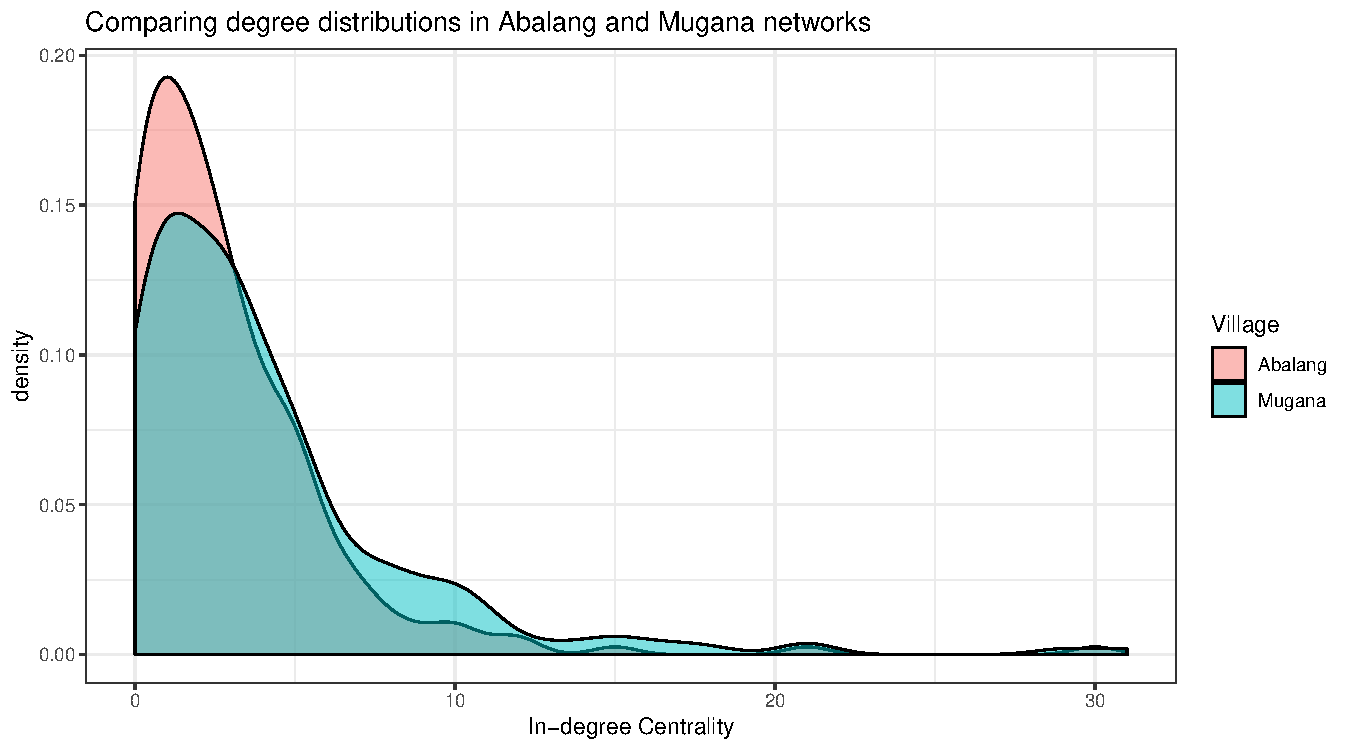
\includegraphics{./figures/degree_comparison.pdf}

The distributions of betweenness centrality in these two networks shows a similar pattern.\footnote{Note to Bruce: an earlier version of this section reported an odd pattern of betweenness centrality that you commented on in the last draft. With subsequent examination, I discovered that this was the result of an error in the code where R was treating the betweenness values as factor levels rather than floats. Upon correction, the pattern is a little less surprising.} Both distributions are right-skewed, and the majority of nodes have low betweenness scores indicating that they are not ``gatekeepers'' to the diffusion of information throughout the network. However, the Abalang distribution has a higher peak, and the Mugana network has a fatter tail, indicating that more nodes in the Mugana network serve as bridges, or potential choke points in the flow of information. 

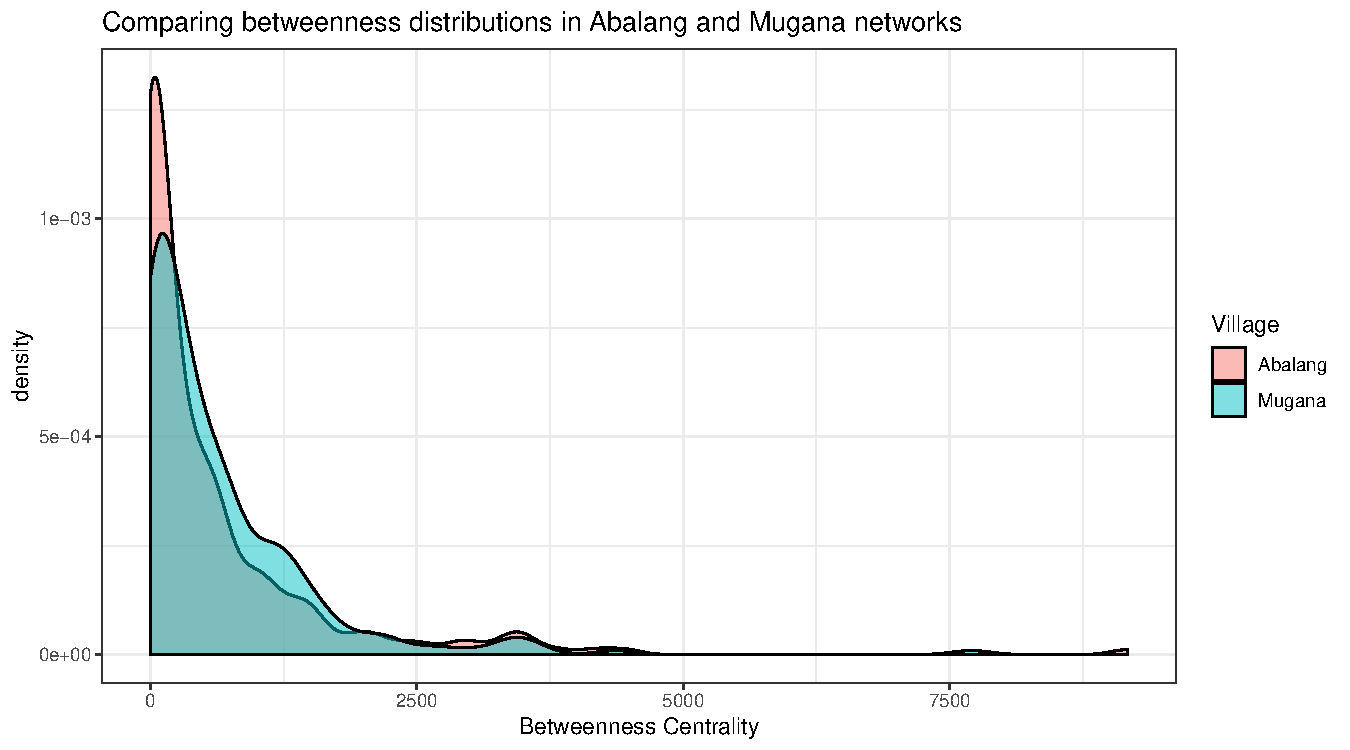
\includegraphics{./figures/betweenness_comparison.pdf}

We can also compare several characteristics of these two networks at the graph level, as shown in the table below:


\begin{table}[!htbp] \centering 
  \caption{Graph-level Descriptive Statistics} 
  \label{} 
\begin{tabular}{@{\extracolsep{5pt}} ccccccc} 
\\[-1.8ex]\hline 
\hline \\[-1.8ex] 
 & Village & density & reciprocity & transitivity & degree\_assortativity & ethnic\_assortativity \\ 
\hline \\[-1.8ex] 
1 & Abalang & $0.013$ & $0.193$ & $0.141$ & $$-$0.004$ & $$ \\ 
2 & Mugana & $0.017$ & $0.196$ & $0.142$ & $0.081$ & $0.183$ \\ 
\hline \\[-1.8ex] 
\end{tabular} 
\end{table} 


First, recalculating the density of the two graphs, we observe as Larson and Lewis did that the Mugana network is denser than the Abalang network. We also see that both of these networks exhibit similar levels of reciprocity and transitivity, indicating that in both villages there are similar tendencies for villagers to send social ties to those from whom they receive ties, and for villagers with mutual ties to themselves be connected. However, when we consider the assortativity of these networks, the similarities end. In the Mugana network, villagers exhibit degree assortativity, indicating that there is a tendency for nodes with similar numbers of ties to seek out connections with each other. In the Abalang network, villagers do not exhibit this tendency, and are actually marginally disassortative by degree. When we consider assortativity by ethnicity, we see that the Mugana network appears to demonstrate a relatively strong tendency for coethnic preferential attachment, suggesting support for H2. However, since the Abalang village is functionally homogeneous, a direct comparison cannot be made, so it remains an open question whether the Mugana network is unique in this regard. This information is displayed visually in the plot below:

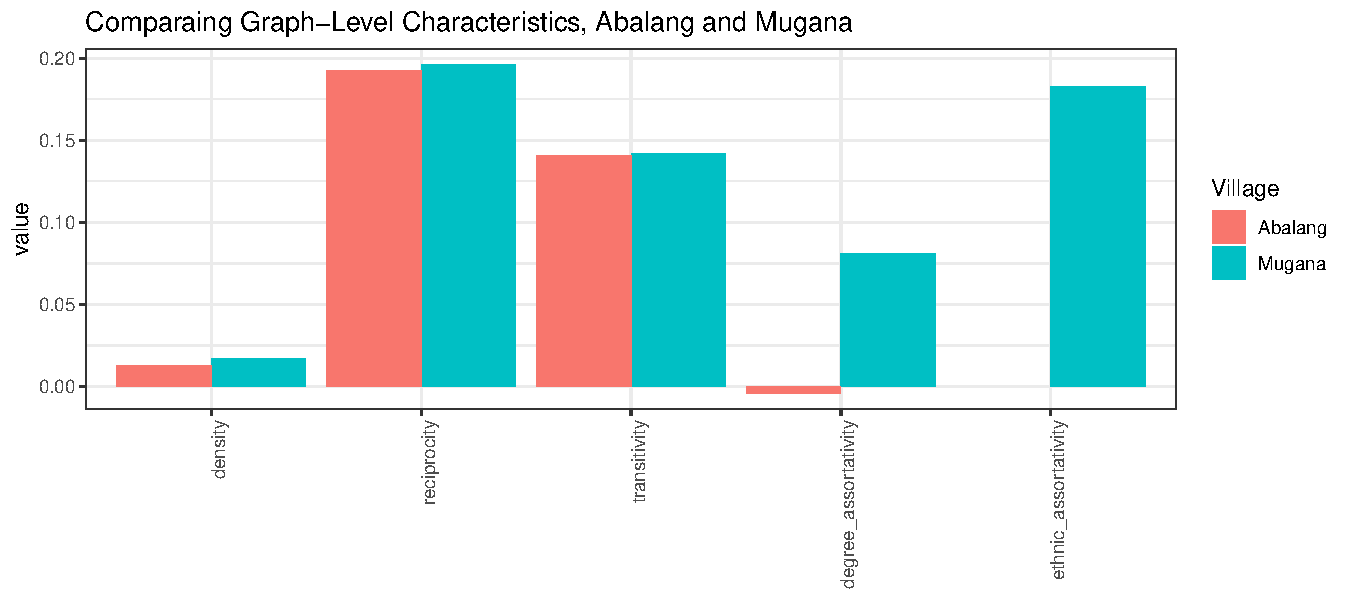
\includegraphics{./figures/graph_characteristics.pdf}

\subsection{ERGM analysis}

The descriptive results reported above are suggestive of support for the hypothesis that ethnically heterogeneous networks are characterized by ethnic preferential attachment, so to evaluate this hypothesis more rigorously, I fit an Exponential Random Graph Model (ERGM) to each network to statistically test the role various network dependencies play in the formation of ties. These models are presented in Table 5 below:


% Table created by stargazer v.5.2.2 by Marek Hlavac, Harvard University. E-mail: hlavac at fas.harvard.edu
% Date and time: Fri, May 01, 2020 - 11:40:11
\begin{table}[!htbp] \centering 
  \caption{ERGM Results for Abalang and Mugana Networks} 
  \label{} 
\begin{tabular}{@{\extracolsep{5pt}}lcc} 
\\[-1.8ex]\hline 
\hline \\[-1.8ex] 
 & \multicolumn{2}{c}{\textit{Dependent variable:}} \\ 
\cline{2-3} 
\\[-1.8ex] & abnet & munet \\ 
\\[-1.8ex] & (1) & (2)\\ 
\hline \\[-1.8ex] 
 edges & $-$4.075$^{***}$ (0.189) & $-$3.834$^{***}$ (0.238) \\ 
  mutual & 3.463$^{***}$ (0.155) & 3.311$^{***}$ (0.131) \\ 
  gwnsp & $-$0.158$^{***}$ (0.020) & $-$0.187$^{***}$ (0.014) \\ 
  gwnsp.decay & $-$1.086$^{***}$ (0.239) & $-$1.219$^{***}$ (0.047) \\ 
  idegree0 & 1.853$^{***}$ (0.235) & 2.242$^{***}$ (0.266) \\ 
  gwodegree & $-$1.104$^{***}$ (0.240) & $-$0.734$^{***}$ (0.259) \\ 
  gwodegree.decay & 0.304 (0.271) & 0.660 (0.429) \\ 
  nodeifactor.Tribe.ATESO & 0.114 (0.238) & 0.443$^{*}$ (0.228) \\ 
  nodeifactor.Tribe.KUMAM &  & 0.584$^{***}$ (0.223) \\ 
  nodematch.Tribe.ATESO & 0.456$^{**}$ (0.179) & 0.341$^{***}$ (0.079) \\ 
  nodematch.Tribe.KUMAM &  & 0.423$^{***}$ (0.088) \\ 
 \hline \\[-1.8ex] 
Akaike Inf. Crit. & 6,627.801 & 9,036.178 \\ 
Bayesian Inf. Crit. & 6,707.330 & 9,134.429 \\ 
\hline 
\hline \\[-1.8ex] 
\textit{Note:}  & \multicolumn{2}{r}{$^{*}$p$<$0.1; $^{**}$p$<$0.05; $^{***}$p$<$0.01} \\ 
\end{tabular} 
\end{table} 


Several covariates from these models are worth discussing. First of these is \textit{mutual}, which captures reciprocity in directed networks. The descriptive measures of reciprocity reported above suggested that both networks were similarly reciprocal at a high level. The ERGM analysis confirms this, with similar positive and significant coefficients for \textit{mutual} in both models, indicating that both networks exhibit greater reciprocity than would be expected if ties were distributed at random. To account for transitivity in the network, I include the \textit{gwnsp} term which captures the prevalence of shared partners between nodes.\footnote{I tried to use \textit{gwesp} here, but the models became degenerate and/or would not converge. My understanding of \textit{gwnsp} is that it captures non-edgewise shared partners--would this be anti-transitivity?}  To account for popularity effects, I include the \textit{gwodegree} term.\footnote{My intention here was to capture preferential attachment by degree, which I understand can be model in undirected networks using \textit{gwdegree}. Since this is a directed network, I tried to include both \textit{gwidegree} and \textit{gwodegree}, but again the models would not converge with these specifications}. Finally, these ERGMs also capture the effects of node-level ethnicity on tie formation. First, using \textit{nodeifactor}, I control for the tendency of certain ethnic identities to systematically receive more ties than others. For example, if ethnic fractionalization is high, and one group is much larger than others, we might expect to see outgroup nodes receiving fewer ties. In the Abalang network, there does not appear to be any evidence that Itesos are more likely to receive ties than villagers from other ethnicities. However, in the Mugana network, both Itesos and Kumams are more likely to receive ties than other ethnicities (significant at $p<0.1$ and $p<0.01$ respectively). Using \textit{nodematch}, I test for ethnic assortativity in these networks as well, with several interesting results. First, in both models we observe a significant tendency for Itesos to send ties to each other. Likewise, in the Mugana network, we observe a similar tendency for Kumams to send ties to each other as well. Together, these findings provide support for H2, that these social networks are characterized by preferential attachment by ethnicity. 

\newpage %This line creates a new page for your bibliography.

\pagestyle{empty} % This tells LaTeX to make the bibliography without numbers.
\bibliographystyle{apsr} % This points LaTeX to your bibliography style file - ours is called apsr
\bibliography{replication.bib} % This points LaTeX to your JabRef bibliography database.

\newpage
\appendix

\section{Appendix: ERGM diagnostics}

MCMC samples converged for both models as specified, and neither one exhibits obvious degeneracy. However, I was unable to specify the exact ERGM terms I thought were most theoretically relevant (see footnotes 2 and 3 above). This may contribute to the not-quite-perfect goodness of fit we observe for both models, shown in the GOF boxplots below. First, both models appear to be capturing the out degree and minimum geodesic distance of the observed networks quite well. The in degree distribution, however, is captured relatively poorly, particularly at the low end of the distribution. I tried to correct this by using the \textit{idegree} term to model in degree values that were not being accurately modeled. With this specification, however, the models again failed to converge. Finally, the ERGMs seem to be missing on edge-wise shared partners as well, likely due to the fact that I was unable to get converging models while using the \textit{gwesp} term.

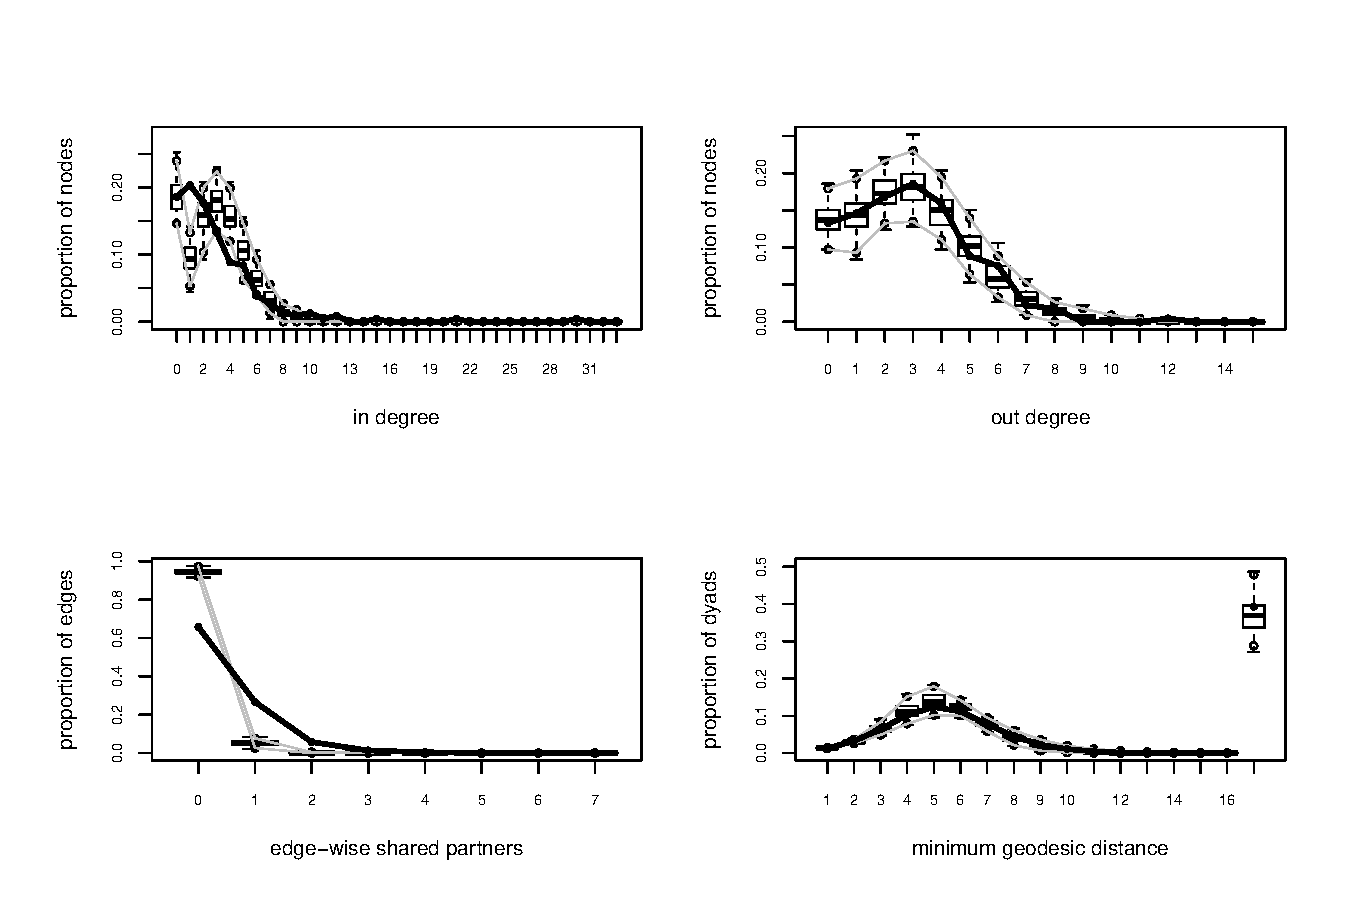
\includegraphics{./figures/abalang_gof.pdf}

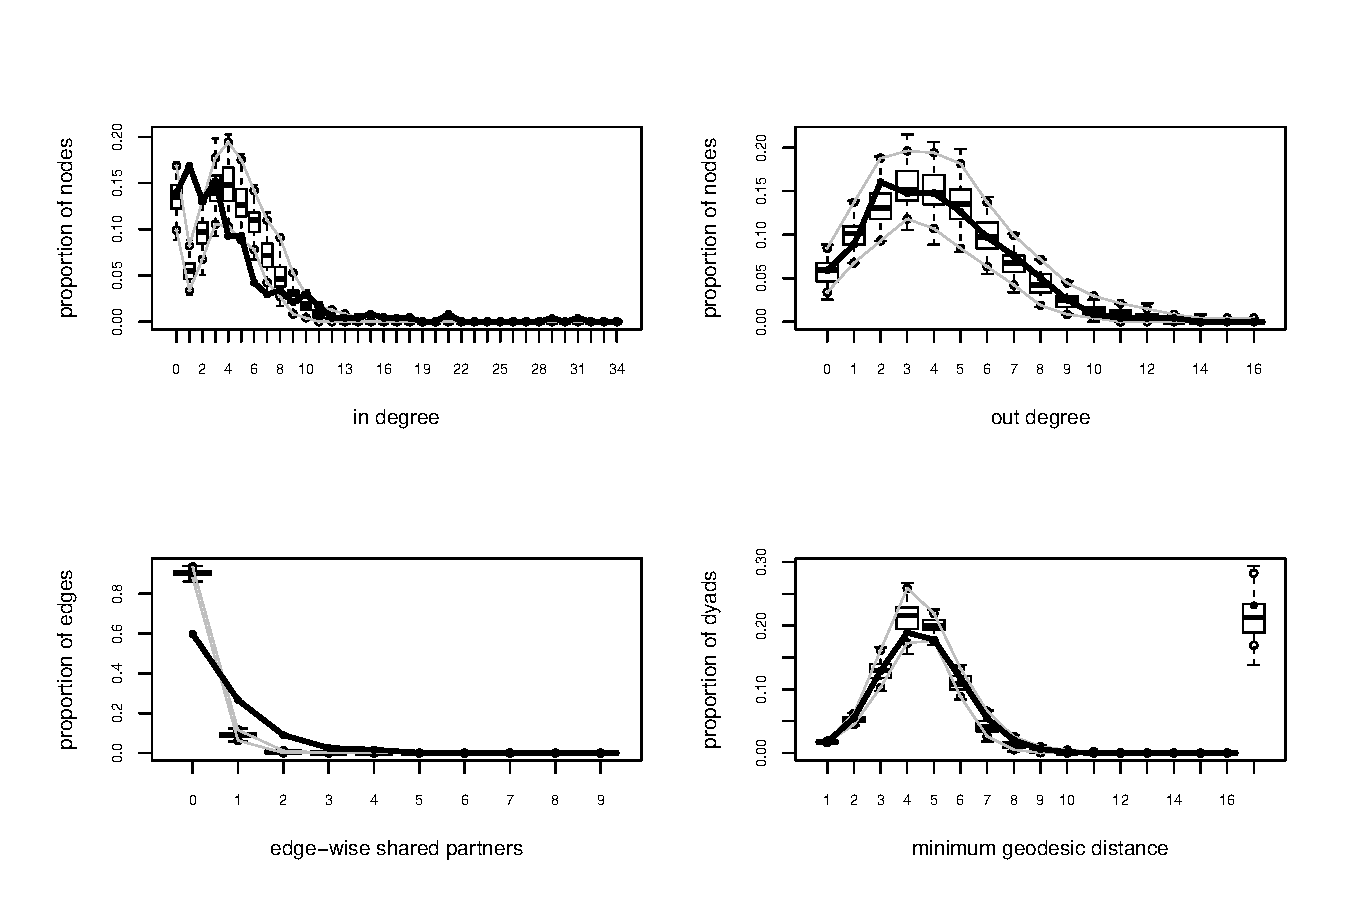
\includegraphics{./figures/mugana_gof.pdf}


\end{document}
